% filepath: fixed_poster.tex
\documentclass[a0,landscape]{ImperialPoster}
\usepackage{graphicx}
\usepackage{multicol}
\usepackage{amsmath,amssymb}
\usepackage{booktabs}
\usepackage{tikz}
\usepackage{pgfplots}
\usepackage{adjustbox}
\pgfplotsset{compat=1.18}
\usetikzlibrary{positioning,shapes,arrows,fit,calc,backgrounds}

% Set Imperial colors and custom colors
\definecolor{ICLBlue}{RGB}{0,62,116}
\definecolor{cwDecoy}{RGB}{243,156,18}
\definecolor{cwAlert}{RGB}{231,76,60}
\definecolor{cwFlow}{RGB}{52,152,219}
\definecolor{cwReal}{RGB}{46,204,113}
\definecolor{cwBorder}{RGB}{44,62,80}

% Custom commands for key metrics
\newcommand{\alertignored}{67\%}
\newcommand{\decoyrate}{76.3\%}
\newcommand{\protectrate}{89.4\%}
\newcommand{\latencyppo}{2.3}
\newcommand{\supervisor}[1]{\def\@supervisor{#1}}

% Improve spacing
\setlength{\columnsep}{1.5cm}
\setlength{\parskip}{0.5cm}

\title{AI-Driven Cyber Defense: 89\% Better Protection Through Adaptive Deception}
\author{Miracle Akanmode}
%\supervisor{Kelly Zhang}

\begin{document}
\titlesection

\begin{multicols}{4}

% COLUMN 1 - Problem & Background
\section{The Cyber Challenge}

\textbf{Asymmetric Advantage:} Attackers need to find one vulnerability; defenders must protect everything

\textbf{Alert Fatigue:} \alertignored{} of alerts ignored due to volume

\textbf{Static Defenses Fail:} Traditional defenses remain static while attackers continuously adapt

\begin{center}
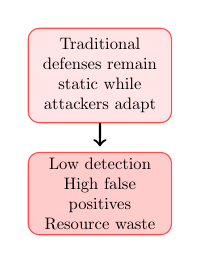
\begin{tikzpicture}[scale=0.6, transform shape]
    % Traditional static defense
    \node[draw=red!70, fill=red!10, rounded corners, minimum width=3cm, minimum height=2cm, text width=2.8cm, align=center] (static) at (0,0) {
        Traditional defenses remain static while attackers adapt
    };
    
    % Arrow pointing down
    \draw[->, thick] (static) -- +(0,-1.5);
    
    % Poor results box
    \node[draw=red!70, fill=red!20, rounded corners, minimum width=3cm, minimum height=1cm, text width=2.8cm, align=center] at (0,-2.5) {
        Low detection\\
        High false positives\\
        Resource waste
    };
\end{tikzpicture}
\end{center}

\section{Research Aim}

Our research addresses this challenge through reinforcement learning agents that:

\begin{itemize}
\item Continuously adapt decoy placement based on observed attack patterns
\item Learn strategic positioning through trial and error
\item Counter adversarial learning
\item Optimize resource allocation
\end{itemize}

This represents a fundamental shift from reactive, static defense toward proactive, adaptive defense that evolves as quickly as the threats it faces.

% COLUMN BREAK
\columnbreak

% COLUMN 2 - Method
\section{Method}
\makeatletter
\let\@noitemerr\relax
\makeatother

\begin{center}
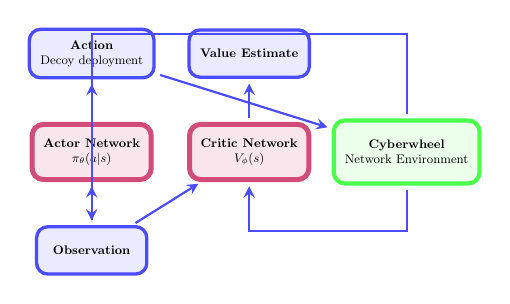
\begin{tikzpicture}[
    node distance=3cm,
    main/.style={draw=blue!70, rounded corners=4pt, fill=blue!8, 
                 inner sep=8pt, minimum width=2.8cm, minimum height=1.2cm, 
                 align=center, font=\small, line width=1.2pt},
    network/.style={draw=purple!70, rounded corners=4pt, fill=purple!10, 
                   inner sep=8pt, minimum width=2.8cm, minimum height=1.4cm, 
                   align=center, font=\small, line width=1.8pt},
    env/.style={draw=green!70, rounded corners=4pt, fill=green!8, 
               inner sep=8pt, minimum width=3cm, minimum height=1.6cm, 
               align=center, font=\small, line width=1.5pt},
    reward/.style={draw=orange!70, rounded corners=4pt, fill=orange!10, 
                   inner sep=8pt, minimum width=3.2cm, minimum height=1.2cm, 
                   align=center, font=\small, line width=1.5pt},
    flow/.style={-stealth, thick, blue!70, shorten >=2pt, shorten <=2pt},
    scale=0.5, transform shape
]

% Actor-Critic Architecture
\node[network] (actor) at (0,0) {\textbf{Actor Network}\\$\pi_\theta(a|s)$};
\node[network] (critic) at (4,0) {\textbf{Critic Network}\\$V_\phi(s)$};

% Inputs and outputs
\node[main] (state) at (0,-2.5) {\textbf{Observation}};
\node[main] (action) at (0,2.5) {\textbf{Action}\\Decoy deployment};
\node[main] (value) at (4,2.5) {\textbf{Value Estimate}};

% Environment
\node[env] (env) at (8,0) {\textbf{Cyberwheel}\\Network Environment};

% Forward flows
\draw[flow] (state) -- (actor);
\draw[flow] (state) -- (critic);
\draw[flow] (actor) -- (action);
\draw[flow] (critic) -- (value);
\draw[flow] (action) -- (env);

% Feedback flow
\draw[flow] (env) -- ++(0,3) -- ++(-8,0) -- (state);
\draw[flow] (env) -- ++(0,-2) -- ++(-4,0) -- (critic);

\end{tikzpicture}
\end{center}

\subsection{Proximal Policy Optimization (PPO)}

We use PPO to train defensive agents with these advantages:
\begin{itemize}
\item Stable learning with clipped surrogate objective
\item Optimized exploration-exploitation balance
\item Sample efficient learning from limited interactions
\end{itemize}

\textbf{Reward Structure:} $R_t = 10 \cdot v_r \cdot \mathbf{1}[\mathrm{decoy~hit}] - v_r \cdot \mathbf{1}[\mathrm{asset~hit}] - 2 \cdot \mathbf{1}[\mathrm{deploy}] - \mathbf{1}[\mathrm{remove}]$

\subsection{Environment}

\begin{center}
\begin{tikzpicture}[
    scale=0.4, transform shape,
    host/.style={circle, draw=blue!60, fill=blue!15, minimum size=7mm, thick},
    decoy/.style={circle, draw=orange!70, fill=orange!15, minimum size=7mm, thick, dashed},
    compromised/.style={circle, draw=red!70, fill=red!20, minimum size=7mm, thick},
    subnet/.style={rectangle, draw=gray!60, fill=gray!8, minimum width=20mm, minimum height=12mm, rounded corners=2pt, align=center},
    agent/.style={rectangle, draw=black, fill=yellow!15, minimum width=18mm, minimum height=10mm, rounded corners=2pt, align=center},
    firewall/.style={rectangle, draw=red!80, fill=red!20, minimum width=8mm, minimum height=15mm, align=center}
]

% Network subnets
\node[subnet] (subnet1) at (-5, 4.5) {DMZ};
\node[subnet] (subnet2) at (-1, 4.5) {Internal};  
\node[subnet] (subnet3) at (3, 4.5) {Critical};

% Hosts
\node[host] (h1) at (-5.5, 5) {$h_1$};
\node[decoy] (d1) at (-4.5, 5) {$d_1$};
\node[host] (h2) at (-1.5, 5) {$h_2$};
\node[compromised] (h3) at (-0.5, 5) {$h_3$};
\node[host] (h4) at (2.5, 5) {$h_4$};
\node[host] (h5) at (3.5, 5) {$h_5$};

% Agents
\node[agent, fill=red!15] (red) at (-5, 1.5) {\mathrm{Red Agent}\\Fixed $\pi^{(r)}$};
\node[agent, fill=blue!15] (blue) at (3, 1.5) {\mathrm{Blue Agent}\\PPO $\pi^{(b)}$};

% Key interactions
\draw[->, thick, blue!70] (blue) to[out=120, in=270] (d1) node[midway, right] {deploy};
\draw[->, thick, red!70, dashed] (red) to[out=60, in=270] (h3) node[midway, left] {attack};

\end{tikzpicture}
\end{center}

\textbf{Environment Features:}
\begin{itemize}
\item Realistic network topology with multiple subnets
\item MITRE ATT\&CK-based adversary modeling
\item Variable scales: 15-200 hosts, 3-8 subnets
\item Deployable honeypots/decoys
\end{itemize}

% COLUMN BREAK
\columnbreak

% COLUMN 3 - Results
\section{Results}

\begin{center}
\Large{\textbf{89\%}}\\
\normalsize{Improvement over static defense}
\end{center}

\begin{center}
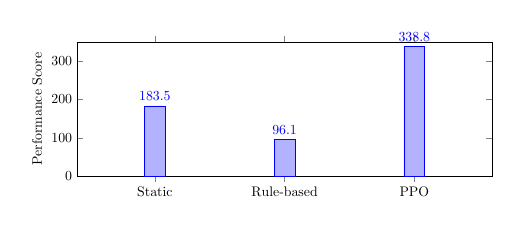
\begin{tikzpicture}[scale=0.5, transform shape]
\begin{axis}[
    width=\textwidth,
    height=5cm,
    ybar,
    bar width=15pt,
    ylabel={Performance Score},
    symbolic x coords={Static,Rule-based,PPO},
    xtick=data,
    ymin=0, ymax=350,
    nodes near coords,
    enlarge x limits=0.3,
]
\addplot coordinates {
    (Static,183.5)
    (Rule-based,96.1)
    (PPO,338.8)
};
\end{axis}
\end{tikzpicture}
\end{center}

\subsection{Security Metrics}

\begin{center}
\begin{tabular}{@{}lccc@{}}
\toprule
\textbf{Metric} & \textbf{PPO} & \textbf{Static} & \textbf{Rule} \\
\midrule
Deception Rate & \decoyrate & 45.1\% & 32.4\% \\
Protection Rate & \protectrate & 61.7\% & 48.2\% \\
Detection Latency & \latencyppo & 4.1 & 5.8 \\
\bottomrule
\end{tabular}
\end{center}

\subsection{Performance Analysis}

\begin{center}
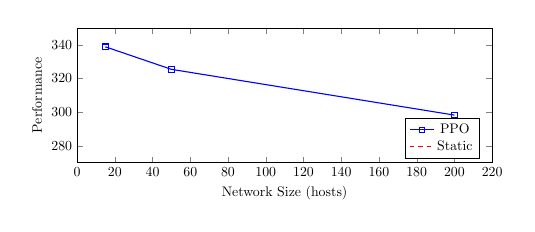
\begin{tikzpicture}[scale=0.5, transform shape]
\begin{axis}[
    width=\textwidth,
    height=5cm,
    xlabel={Network Size (hosts)},
    ylabel={Performance},
    xmin=0, xmax=220,
    ymin=270, ymax=350,
    legend pos=south east,
]
\addplot[thick, blue, mark=square] coordinates {
    (15, 338.8)
    (50, 325.4)
    (200, 298.2)
};
\addplot[thick, red, dashed] coordinates {
    (15, 183.5)
    (50, 179.2)
    (200, 172.6)
};
\legend{PPO, Static}
\end{axis}
\end{tikzpicture}
\end{center}

\begin{center}
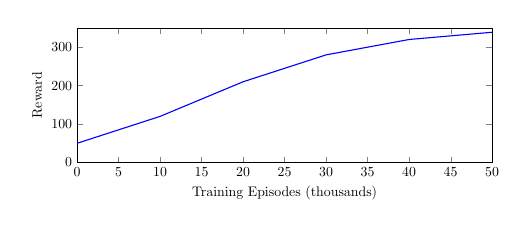
\begin{tikzpicture}[scale=0.5, transform shape]
\begin{axis}[
    width=\textwidth,
    height=5cm,
    xlabel={Training Episodes (thousands)},
    ylabel={Reward},
    xmin=0, xmax=50,
    ymin=0, ymax=350,
]
\addplot[thick, blue] coordinates {
    (0, 50) (10, 120) (20, 210) 
    (30, 280) (40, 320) (50, 338.8)
};
\end{axis}
\end{tikzpicture}
\end{center}

% COLUMN BREAK
\columnbreak

% COLUMN 4 - Strategic Behavior, Conclusions
\section{Strategic Behavior}

\begin{center}
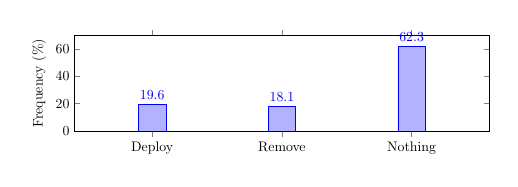
\begin{tikzpicture}[scale=0.5, transform shape]
\begin{axis}[
    width=\textwidth,
    height=4cm,
    ybar,
    bar width=20pt,
    ylabel={Frequency (\%)},
    symbolic x coords={Deploy,Remove,Nothing},
    xtick=data,
    ymin=0, ymax=70,
    nodes near coords,
    enlarge x limits=0.3,
]
\addplot coordinates {
    (Deploy,19.6)
    (Remove,18.1)
    (Nothing,62.3)
};
\end{axis}
\end{tikzpicture}
\end{center}

\textbf{Emergent Intelligence:} The PPO agent demonstrates strategic restraint, choosing "no action" 62\% of the time. This shows the agent has learned that excessive decoy deployment is counterproductive and strategically balances security needs with resource costs.

\begin{center}
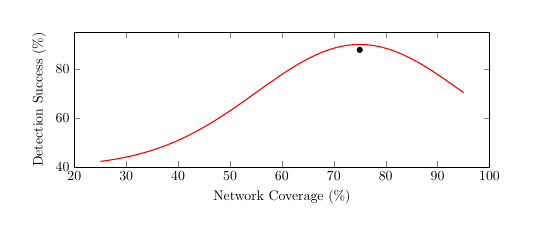
\begin{tikzpicture}[scale=0.5, transform shape]
\begin{axis}[
    width=\textwidth,
    height=5cm,
    xlabel={Network Coverage (\%)},
    ylabel={Detection Success (\%)},
    xmin=20, xmax=100,
    ymin=40, ymax=95,
]
% Performance curve with optimal point
\addplot[thick, red, domain=25:95, samples=50] {40 + 50*exp(-(x-75)^2/800)};
\addplot[mark=*, only marks] coordinates {(75, 87.8)};
\end{axis}
\end{tikzpicture}
\end{center}

\section{Conclusion}

\textbf{Key Findings:}
\begin{itemize}
\item PPO learns adaptive defense strategies that outperform static approaches by 89\%
\item Strategic restraint emerges naturally through reinforcement learning
\item Adaptive deception creates uncertainty for attackers, disrupting reconnaissance and lateral movement
\item Performance scales effectively to enterprise networks (up to 200 hosts tested)
\end{itemize}

\textbf{Future Work:}
\begin{itemize}
\item Adversarial co-evolution of attack and defense strategies
\item Multi-objective optimization balancing security with resource constraints
\item Real-world deployment testing
\item Transfer learning across network topologies
\end{itemize}

\vspace{1cm}

\section{Contact \& References}

\textbf{Miracle Akanmode}\\
miracle.akanmode24@imperial.ac.uk\\
Imperial College London\\
Supervisor: Dr. Kelly Zhang

\end{multicols}
\end{document}